\documentclass[11pt, oneside]{book}		%	Visualize as PDF
%\documentclass[11pt]{book}				%	To be printed

\usepackage[utf8]{inputenc}
\usepackage[spanish]{babel}
\usepackage{graphicx}
\usepackage{float}
\usepackage{url}
\usepackage{xcolor}
\usepackage{listingsutf8}
\usepackage[hidelinks]{hyperref}
\usepackage{accsupp}
\usepackage{etoolbox}

\renewcommand*{\thelstnumber}{\protect\BeginAccSupp{ActualText={}}\arabic{lstnumber}\protect\EndAccSupp{}}
\AtBeginDocument{\renewcommand*{\theHlstnumber}{\arabic{lstnumber}}}
\makeatletter
	\patchcmd{\lst@GLI@}% <command>
	{\def\lst@firstline{#1\relax}}% <search>
	{\def\lst@firstline{#1\relax}\def\lst@firstnumber{#1\relax}}% <replace>
	{\typeout{listings firstnumber=firstline}}% <success>
	{\typeout{listings firstnumber not set}}% <failure>
\makeatother

\definecolor{bluekeywords}{rgb}{0.349,0.635,0.8}
\definecolor{lightgreenkeywords}{rgb}{0.356,0.752,0.631}
\definecolor{yellowgreenkeywords}{rgb}{0.756,0.831,0.670}
\definecolor{greencomments}{rgb}{0,0.5,0}
\definecolor{orangestrings}{rgb}{0.823,0.568,0.439}
\definecolor{types}{rgb}{0.17,0.57,0.68}
\definecolor{background}{rgb}{0.117,0.117,0.117}

\title{Bases de la programación (\textit{C}\#)}
\author{Carlos Clement Bellido}
\date{\today}

\hypersetup{
	colorlinks=true,
	linkcolor=blue,
	linktocpage=true
}

\lstset{language=csh,
		captionpos=b,
		frame=shadowbox,
		rulecolor=\color{blue},
		rulesepcolor=\color{blue},
		linewidth=16.2cm,
		%morecomment = [l]{//},
		%morecomment = [s]{/*}{*/},
		commentstyle=\color{greencomments},
		numberstyle=\tiny\color{black},
		numbers=left,
		showspaces=false,
		showtabs=true,
		showstringspaces=false,
		breakatwhitespace=true,
		escapeinside={(*@}{@*)},
		extendedchars=true,
		emph=[1]
		{ 	abstract, event, new, struct,
			as, explicit, null, switch,
			base, extern, object, this,
			bool, false, operator, throw,
			break, finally, out, true,
			byte, fixed, override, try,
			case, float, params, typeof,
			catch, for, private, uint,
			char, foreach, protected, ulong,
			checked, goto, public, unchecked,
			class, if, readonly, unsafe,
			const, implicit, ref, ushort,
			continue, in, return, using,
			decimal, int, sbyte, virtual,
			default, interface, sealed, volatile,
			delegate, internal, short, void,
			do, is, sizeof, while,
			double, lock, stackalloc,
			else, long, static, get,
			enum, namespace, string, set
			},
		emphstyle=[1]\color{bluekeywords},
		emph=[2]
		{	StreamReader, Dictionary, DateTime, Environment,
			Program, Console, Queue, Stack,
			List, StreamWriter, KeyValuePair, Directory,
			File, Rally, Equipo, Interruptor,
			Bombilla},
		emphstyle=[2]\color{lightgreenkeywords},
		emph=[3]
		{	ConsoleKey},
		emphstyle=[3]\color{yellowgreenkeywords},
		stringstyle=\color{orangestrings},
		basicstyle=\ttfamily\small,
		breaklines=true,
		inputencoding=utf8/latin1,
		columns=flexible,
		tabsize=3,
		basicstyle=\ttfamily\color{white},
		backgroundcolor = \color{background},
		xleftmargin=\dimexpr-\leftmarginii-\leftmargini-25pt
}

\pdfinfo{
	/title (Bases de la programacion)
	/author (Carlos Clement Bellido)
}

\begin{document}
	
\maketitle 	
\tableofcontents

\chapter*{Prólogo}
\textbf{Atención: este documento ha sido escrito como forma de apoyo para dar clases, puede que algunas cosas no queden del todo claras o no tengan una definición precisa (intentaré ser lo más claro y conciso posible). No dudes en contactar conmigo para sugerencias, correcciones o lo que se pase por tu mente.}
\begin{center}
	\href{mailto:carlos.clement.bellido@gmail.com}{carlos.clement.bellido@gmail.com}
\end{center}
Algún rollo sobre la programación en inglés\\
Si es tu primer contacto con la programación, tómatelo con paciencia y no te rindas, lo que se te viene encima no es sencillo. \textit{Si vis pacem, para bellum}.
\addcontentsline{toc}{chapter}{Prólogo}

%\chapter{Tipos básicos}
%	\section{Entero (\textit{int})}
%\section{Funciones}
\chapter{Tipos enumerables}
	\section{Matriz (\textit{array})}
	Las matrices, o \textit{arrays}\cite{msdn:array}, son agrupaciones de un determinado número elementos del mismo tipo. La cuantía ha de definirse en la inicialización de la matriz y, por lo general, no se alterará. Tenemos tres tipos básicos: la unidimensional, que es la más común de ver, la multidimensional, la cual nos permitirá trabajar con varias dimensiones, y la escalonada, que es similar a la multidimensional con la salvaguarda de que no se requiere que todas las dimensiones tengan el mismo tamaño.\\
	Un concepto muy importante a tener en cuenta es que tenemos que comprender que \textbf{una matriz es un tipo de datos} también.
		\subsection{Unidimensional}
		En una matriz unidimensional\cite{msdn:matrizunidimensional} cada dato le corresponde a un índice, que será un número. De este modo, podemos añadir datos a la matriz (siempre y cuando haya espacios libres).\\
		Pongamos el ejemplo de que queremos guardar los nombres de los tres primeros pilotos que llegan a meta. Sabemos que siempre tendremos que guardar tres nombres, así que de primeras inicializamos la matriz: 
		\begin{figure}[H]
			\centering
			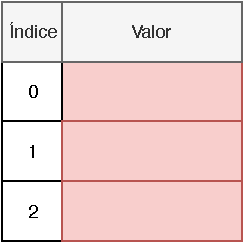
\includegraphics{img/TiposEnumerables/Matriz/array1.pdf}
		\end{figure}
		Los valores que guardemos serán de un tipo determinado; como en este caso guardaremos nombre de pilotos, el tipo de datos sera un tipo cadena (\textit{string}). Los tres pilotos que queremos meter serán:
		\begin{enumerate}
			\item Carlos Sainz
			\item Colin McRae
			\item Dani Sordo
		\end{enumerate}
		Así que, uno a uno, los insertaremos hasta que rellenemos la matriz.
		\begin{figure}[H]
			\centering
			\hspace*{-0.3in}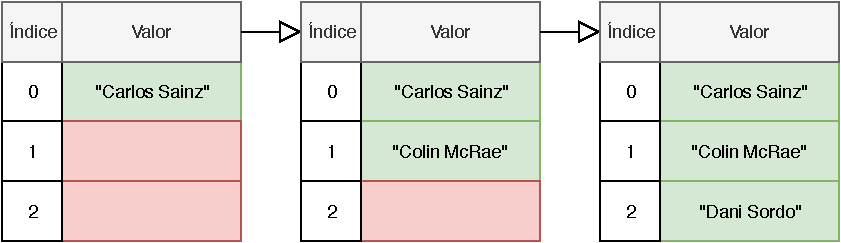
\includegraphics{img/TiposEnumerables/Matriz/array2.pdf}
		\end{figure}
		De izquierda a derecha, cada piloto le corresponde la posición en la que ha quedado. Si Carlos Sainz ha quedado primero, le corresponderá el 0; esto es debido a que \textbf{los índices comienzan en 0}.\\
		Podremos acceder a los elementos del interior de la matriz refiriéndonos a ellos por su índice.
		\\\\\begin{minipage}[c]{0.95\textwidth}
			\lstinputlisting[language=csh,firstline=13,lastline=20]{Programas/Matriz/Program.cs}
		\end{minipage}
		En la primera declaración definimos el tamaño de la matriz introduciendo los datos; de este modo sabemos que la matriz es de 2 elementos. En la segunda declaración indicamos que la matriz tiene 3 elementos y no hay nada en esos índices (nada que el usuario haya puesto).
		\subsection{Multidimensional}
		Si comprendemos la matriz unidimensional y el hecho de que una matriz es un tipo de dato, entonces podremos entender que una matriz multidimensional\cite{msdn:matrizmultidimensional} es una matriz de matrices.
		\begin{figure}[H]
			\centering
			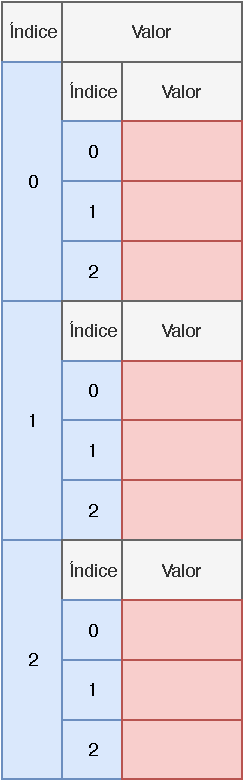
\includegraphics{img/TiposEnumerables/Matriz/array3.pdf}
		\end{figure} 
		Accedemos a cada elemento por cada uno de sus índices. Apréciese que no es posible que dos elementos tengan el mismo índice. También vemos que es una matriz de 3 dimensiones y por cada dimensión tenemos tres elementos\\
		En el siguiente ejemplo guardamos números en cada uno de las matrices:
		\begin{figure}[H]
			\centering
			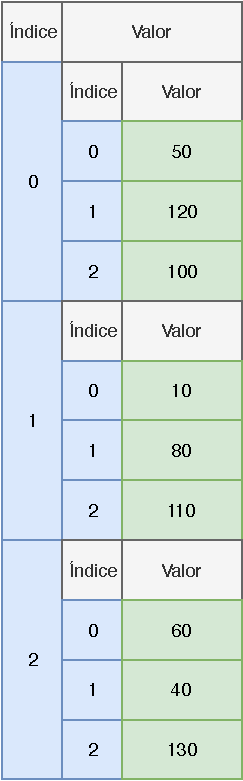
\includegraphics{img/TiposEnumerables/Matriz/array4.pdf}
		\end{figure} 
		Apréciese que si queremos acceder a un dato, mediante el índice de las matrices podemos acceder a él. Por ejemplo, si queremos saber lo que hay en el índice (1, 0) obtendremos <<10>>.\\
		Para plasmar esta matriz en código podremos hacerlo de las siguientes formas:
		\\\\\begin{minipage}[c]{0.95\textwidth}
			\lstinputlisting[language=csh,firstline=22,lastline=43]{Programas/Matriz/Program.cs}
		\end{minipage}
		\subsection{Escalonada (\textit{jagged})}
		Una matriz escalonada\cite{msdn:matrizescalonada} es muy similar a la multidimensional, pero no es necesario que las matrices contenidas en la matriz sean todas de la misma dimensión.
		\begin{figure}[H]
			\centering
			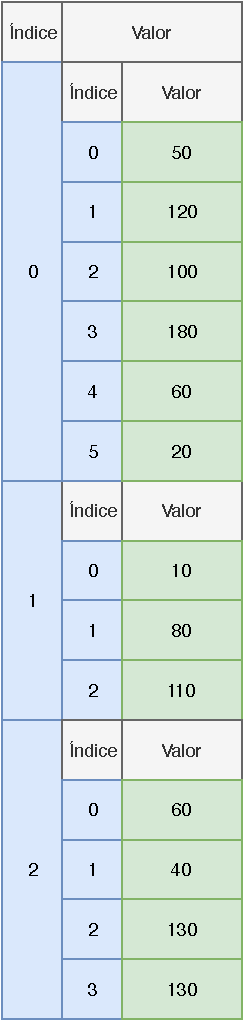
\includegraphics{img/TiposEnumerables/Matriz/array5.pdf}
		\end{figure}
		En la figura superior tenemos una matriz que agrupa tres matrices, cada una de ellas de diferente longitud. Al igual que en la multidimensional, accedemos a los datos mediante los dos índices; por ejemplo, en la posición (2,3) tenemos el número <<130>>.\\
		Dicha matriz se vería en código de las siguientes formas:
		\\\\\begin{minipage}[c]{0.95\textwidth}
			\lstinputlisting[language=csh,firstline=45,lastline=83]{Programas/Matriz/Program.cs}
		\end{minipage}
	\section{Lista}
	Una lista\cite{msdn:lista} posee la misma función que una matriz, almacenar datos del mismo tipo. Con respecto de las matrices podemos destacar dos aspectos; uno favorable y otro desfavorable:
	\begin{itemize}
		\item No tenemos un tamaño fijo, pueden agrandarse cuanto se quiera.
		\item El tiempo de acceso a los valores aumenta debido a que no accedemos a los elementos mediante un índice. Esto es que las listas solo permiten un acceso secuencial a los elementos mientras que las matrices puede ser un acceso aleatorio.
	\end{itemize}
	Una lista consta, principalmente, de los siguientes datos:
	\begin{itemize}
		\item Valor: este sera el valor que queremos guardar.
		\item Siguiente elemento: este campo será una referencia al elemento siguiente. Cada uno de los elementos de nuestra lista tendrá una referencia al elemento que le sigue. Para obtener cualquiera de los valores solo tenemos que conocer la posición del primer elemento e ir recorriendo de elemento en elemento.
	\end{itemize}
	Cabe destacar que una lista puede tener también un elemento que sea <<Elemento anterior>>, y nos sirva para recorrer la lista en dos direcciones.\\
	De hecho, tenemos varias posibilidades de listas que veremos en las siguientes subsecciones.\\
	Pese a todos los tipos de listas, en \textit{(C\#} trabajaremos con una principalmente, \textit{List \textless T\textgreater}. Para definir una lista de nombres podremos hacerlo tal que así:
	\\\\\begin{minipage}[c]{0.95\textwidth}
		\lstinputlisting[language=csh,firstline=13,lastline=17]{Programas/Lista/Program.cs}
	\end{minipage}
		\subsection{Simplemente enlazada}
		Cada elemento apunta al que le sigue o le precede. Lo normal es que apunte al que le sucede.
		\begin{figure}[H]
			\centering
			\hspace*{-0.9in}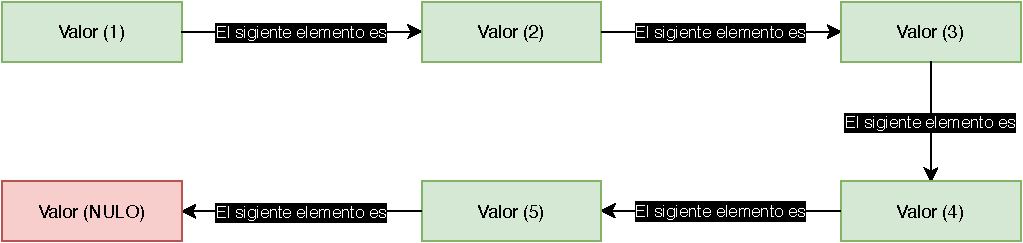
\includegraphics{img/TiposEnumerables/Lista/list1.pdf}
		\end{figure}
		Como podemos apreciar, el último elemento apunta a nulo. Si queremos ir hasta el final de la lista habremos de empezar a recorrer la lista desde el primer elemento e ir <<saltando>> de elemento en elemento hasta que el elemento sea nulo; cuando sea nulo, sabremos que hemos llegado al final.\\
		Desde un punto de vista de la memoria se podría ver de la siguiente manera (\textbf{atención, esto no implica que una lista sea guardada así en memoria}):
		\begin{figure}[H]
			\centering
			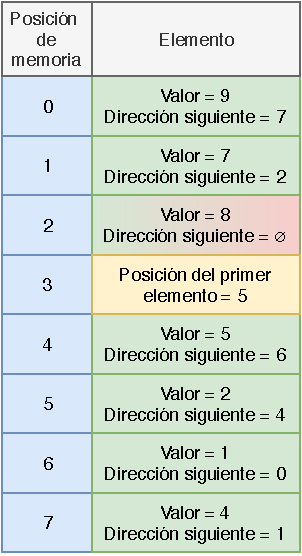
\includegraphics{img/TiposEnumerables/Lista/list1-1.pdf}
		\end{figure}
		En la posición de memoria <<3>> tenemos guardada la posición del primer elemento, y es lo único que conocemos de la lista. Nos está indicando que la lista empieza en la dirección <<5>>, vayámonos a ella. ¿Qué nos encontramos? Que en esta posición tenemos guardado el número 2, que es el dato que queríamos guardar; ahora nos vamos al siguiente elemento, cuya dirección de memoria esta guardada en la misma dirección que acabamos de comprobar: en nuestro caso, la siguiente dirección de memoria es la 4. En la 4 tenemos el valor 5 y el siguiente elemento es el 6. De este modo vamos recorriendo la lista hasta llegar a un elemento que la dirección del siguiente elemento sea nulo. Véase el caso del elemento en la dirección de memoria 2: accedemos a él por medio del elemento que hay en la posición 1, y el siguiente elemento es nulo, es decir, en este elemento (2) acaba la lista.
		\subsection{Doblemente enlazada}
		En este tipo de lista, cada elemento apunta a su siguiente y a su anterior.
		\begin{figure}[H]
			\centering
			\hspace*{-0.9in}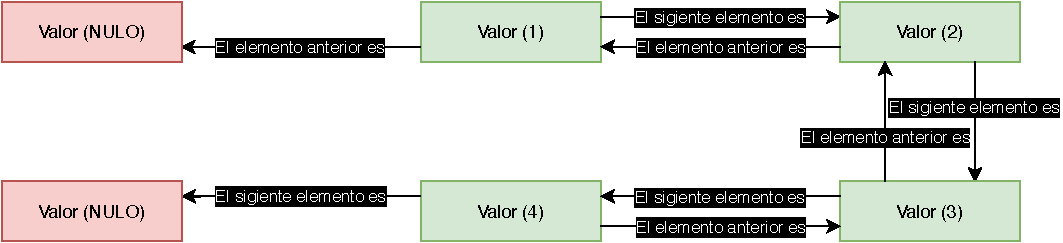
\includegraphics{img/TiposEnumerables/Lista/list2.pdf}
		\end{figure}
		De esta forma podremos recorrer la lista desde el primer elemento hasta el último y desde el último hasta el primero.
		\subsection{Circular}
		No vamos a entrar en detalles con este tipo de lista, pero su peculiaridad es que ninguno de los nodos apunta a nulo: el último apuntará al primero y, en caso de ser doblemente enlazada, el primero apuntará al último (con su puntero a <<anterior>>):
		\begin{figure}[H]
			\centering
			\hspace*{-0.6in}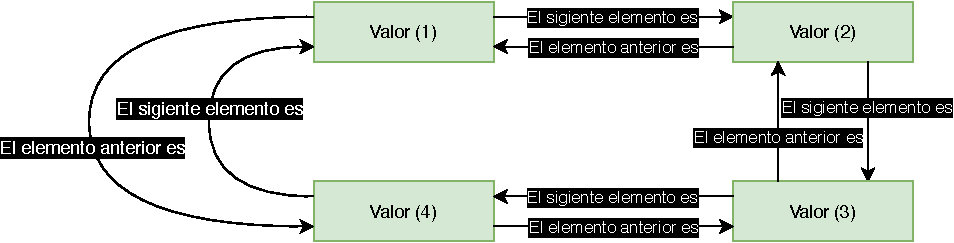
\includegraphics{img/TiposEnumerables/Lista/list3.pdf}
		\end{figure}
	\section{Pila (\textit{stack})}
	Las pilas\cite{msdn:stack} son similares a las listas, pero su peculiaridad es cómo se accede a sus datos. El modo de acceso es de tipo LIFO (\textit{Last In First Out}), es decir, el último en entrar es el primero en salir.
	\begin{figure}[H]
		\centering
		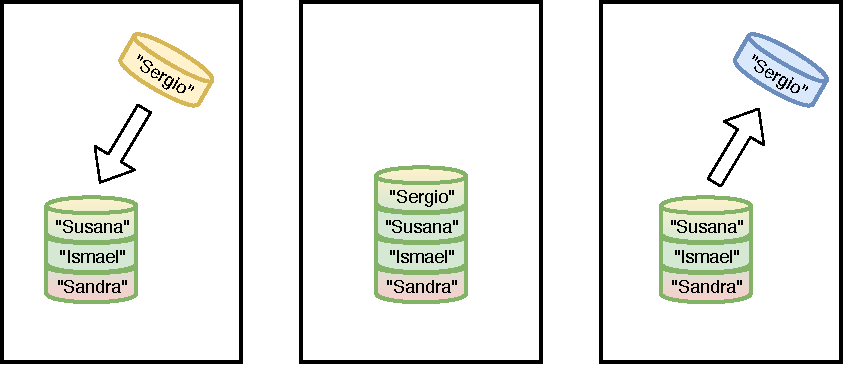
\includegraphics{img/TiposEnumerables/Pila/pila1.pdf}
	\end{figure} 
	En el ejemplo vemos una lista simple de cadenas. El primer elemento que se añadió es <<``Sandra''>>, seguido de <<``Ismael''>> y el último añadido es <<``Susana''>>; Añadimos un elemento más, <<``Sergio''>>, de tal forma que ahora <<``Susana''>> no está en la cima de la pila. En la última imagen sacaremos el último elemento añadido, que es <<``Sergio''>>; de este modo, el siguiente elemento a retirar de la pila es <<``Susana''>>.\\
	El siguiente código es una demostración de la imagen.\\
	Creación de la pila:
	\\\\\begin{minipage}[c]{0.95\textwidth}
		\lstinputlisting[language=csh,firstline=10,lastline=13]{Programas/Pila/Program.cs}
	\end{minipage}
	Adición de la cadena <<``Sergio''>> a la pila:
	\\\\\begin{minipage}[c]{0.95\textwidth}
		\lstinputlisting[language=csh,firstline=15,lastline=15]{Programas/Pila/Program.cs}
	\end{minipage}
	Quitamos el último elemento (<<``Sergio''>>) y lo mostramos; con la última línea solo mostramos el último elemento.
	\\\\\begin{minipage}[c]{0.95\textwidth}
		\lstinputlisting[language=csh,firstline=17,lastline=18]{Programas/Pila/Program.cs}
	\end{minipage}
	De este modo, tendríamos este programa:
	\\\\\begin{minipage}[c]{0.95\textwidth}
		\lstinputlisting[language=csh]{Programas/Pila/Program.cs}
	\end{minipage}
	\section{Cola (\textit{queue})}
	Las colas\cite{msdn:queue} poseen la misma peculiaridad que las pilas: el acceso a los datos es especial. El modo de acceso a datos es FIFO (\textit{First In First Out}), el primero en entrar será el primero en salir.
	\begin{figure}[H]
		\centering
		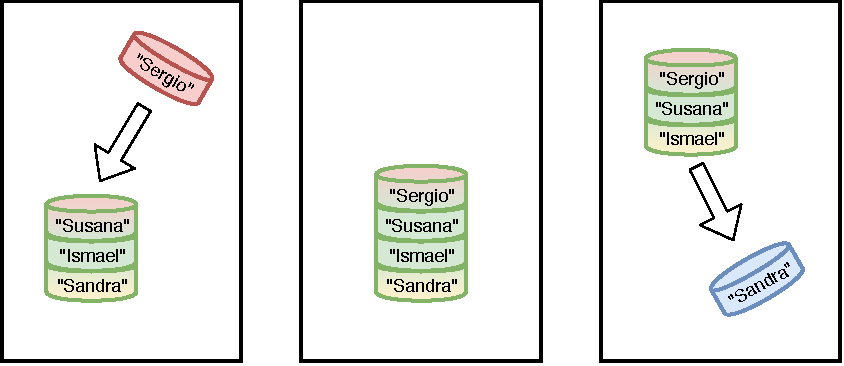
\includegraphics{img/TiposEnumerables/Cola/cola1.pdf}
	\end{figure} 
	Vemos como el primer elemento que se ha añadido es <<``Sandra''>>, por lo tanto dará igual cuántas cosas añadamos, el primero en salir será <<``Sandra''>>. Pese a añadir <<``Sergio''>>, <<``Sandra''>> saldrá la primera, como en la ultima figura indica. Una vez extraída de la cola, el siguiente elemento que le sigue para ser retirado es <<``Ismael''>>.\\
	Veamos un ejemplo\\
	Creación de la cola:
	\\\\\begin{minipage}[c]{0.95\textwidth}
		\lstinputlisting[language=csh,firstline=10,lastline=13]{Programas/Cola/Program.cs}
	\end{minipage}
	Adición de la cadena <<``Sergio''>> a la pila. Este elemento será, de momento, el último en salir:
	\\\\\begin{minipage}[c]{0.95\textwidth}
		\lstinputlisting[language=csh,firstline=15,lastline=15]{Programas/Cola/Program.cs}
	\end{minipage}
	Quitamos el último elemento (<<``Sandra''>>) y lo mostramos; con la última línea solo mostramos el último elemento (<<``Ismael''>>).
	\\\\\begin{minipage}[c]{0.95\textwidth}
		\lstinputlisting[language=csh,firstline=17,lastline=18]{Programas/Cola/Program.cs}
	\end{minipage}
	De este modo, tendríamos este programa:
	\\\\\begin{minipage}[c]{0.95\textwidth}
		\lstinputlisting[language=csh]{Programas/Cola/Program.cs}
	\end{minipage}
	\section{Diccionario}
	Un diccionario\cite{msdn:diccionario} es un tipo muy potente de almacenado de datos pues, al igual que la lista, no tenemos un límite establecido y además el diccionario nos permite agregar una clave por cada dato que añadamos. Dicha clave será de un tipo concreto (determinado por el usuario). Veamos un ejemplo para una mejor comprensión:
	\begin{figure}[H]
		\centering
		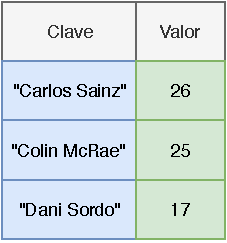
\includegraphics{img/TiposEnumerables/Diccionario/diccionario1.pdf}
	\end{figure} 
	La funcionalidad es muy similar a la de una matriz unidimensional, con la salvaguarda de que lo que sería el índice ahora es una clave. En el ejemplo vemos un diccionario donde los nombres de los pilotos (cadena) son la clave y el valor que les corresponde a cada uno son el número de victorias (número entero). Si buscamos en nuestro diccionario el valor que hay en la clave <<Colin McRae>> nos dará 25.\\
	Con la siguiente linea declaramos el diccionario:
	\\\\\begin{minipage}[c]{0.95\textwidth}
		\lstinputlisting[language=csh,firstline=13,lastline=13]{Programas/Diccionario/Program.cs}
	\end{minipage}
	Podemos agregar elementos de la siguiente forma:
	\\\\\begin{minipage}[c]{0.95\textwidth}
		\lstinputlisting[language=csh,firstline=15,lastline=17]{Programas/Diccionario/Program.cs}
	\end{minipage}	
	Véase que <<``Dani Sordo''>> no tiene las 17 victorias que le corresponden; para modificar un valor en una clave específica lo hacemos con indizadores:
	\\\\\begin{minipage}[c]{0.95\textwidth}
		\lstinputlisting[language=csh,firstline=19,lastline=19]{Programas/Diccionario/Program.cs}
	\end{minipage}	
\chapter{Manejo de directorios}
Antes de ser capaces de entender cómo se manejan los ficheros, hemos de comprender que un fichero está contenido en un \hypertarget{directorioRet}{\hyperlink{directorioDef}{directorio}}\cite{msdn:directorio}.\\
Tanto en este capítulo como en el siguiente (Manejo de ficheros) trabajaremos con el siguiente esquema de directorios y ficheros:
\begin{figure}[H]
	\centering
	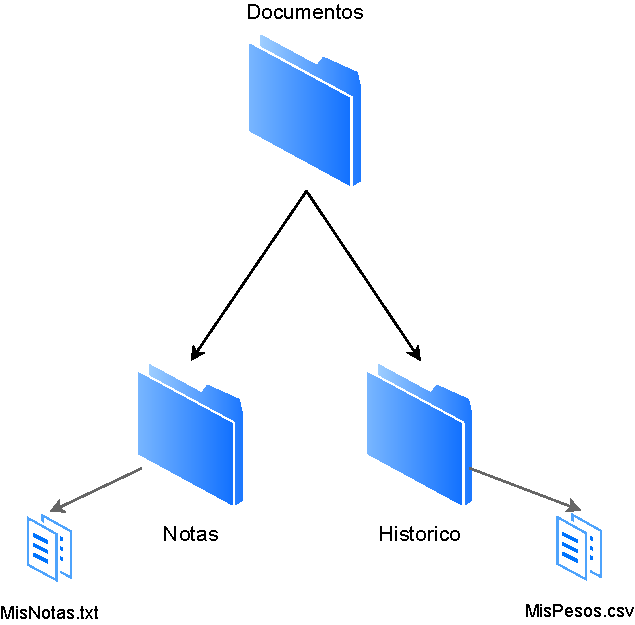
\includegraphics{img/ManejoDeFicherosYDirectorios/esquema.pdf}
\end{figure}
Este será el sistema de archivos de una persona que quiera controlar su peso. Dentro de la carpeta <<Documentos>> tenemos dos carpetas: <<Notas>> e <<Historico>>; nótese que se refiere a <<Hist\textbf{ó}rico>> y por posibles problemas con las tildes hemos decidido suprimirla, pero como siempre digo: \textbf{la programación habría de realizarse toda en inglés}. Dentro del fichero <<Notas>> tendremos <<MisNotas.txt>>, donde el usuario va a guardar notas en relación a alimentación (alimentos que engordan, hábitos saludables, horas para realizar las comidas, etc.). En el otro fichero, <<Historico>>, guardaremos <<MisPesos.csv>>, que será un fichero donde guardaremos de forma ordenada en un \hypertarget{CSVRet}{\hyperlink{CSVDef}{CSV}} con el día y el peso registrado.\\
No usaremos el explorador de archivos para la creación de ninguno de los elementos del árbol.\\
Comenzaremos por la creación de los directorios en el \hypertarget{curdirRet}{\hyperlink{curdirDef}{directorio de nuestro proyecto}}. Con las siguientes lineas creamos los directorios:
\\\\\begin{minipage}[c]{0.95\textwidth}
	\lstinputlisting[language=csh,firstline=14,lastline=17]{Programas/FicherosYDirectorios/Program.cs}
\end{minipage}	
En el caso de estar creados, <<\textit{CreateDirectory}>> no sobreescribirá, simplemente no hará nada: están ya creados.\\
El resto de acciones que pueden hacerse con los directorios, tales como acceder a las propiedades, vienen en el \href{https://docs.microsoft.com/es-es/dotnet/api/system.io.directory?view=netframework-4.8}{MSDN}.
\chapter{Manejo de ficheros}
\textit{C}\# nos proporciona un sistema de manejo de \hypertarget{ficheroRet}{\hyperlink{ficheroDef}{ficheros}}\cite{msdn:fichero} sencillo, el cual desarrollaremos en las siguientes secciones.\\
Tenemos cinco tipos básicos en lo referente a manejo de ficheros:
\begin{itemize}
	\item \textit{Stream}\cite{msdn:stream}: lo usaremos para leer literalmente secuencias de bytes. \textbf{Es necesario para la lectura y la escritura de ficheros}.
	\item \textit{StreamReader}\cite{msdn:streamreader}: podremos leer un fichero caracter a caracter con una \hypertarget{codificacionRet}{\hyperlink{codificacionDef}{codificación}} determinada.
	\item \textit{StreamWriter}\cite{msdn:streamwriter}: semejante al \textit{StreamReader}; podremos escribir en un fichero siempre y cuando los datos a escribir estén codificados correctamente.
	\item \textit{BinaryReader}\cite{msdn:binaryreader}: como bien dice su nombre, lee datos escritos en binario en un fichero.
	\item \textit{BinaryWriter}\cite{msdn:binarywriter}: necesario para la lectura de ficheros binarios. Todos los ficheros son almacenados en binario, pero ello no implica que tengan una decodificación estándar. Podemos guardar 8 bits y cada uno de los valores de cada bit represente un dato concreto. Por ejemplo:
	\\AQUÍ IRÍA UNA FIGURA TO LO GUAPA POSIBLE DE UN FLAG DE UN VIDEOJUEGO QUE VA A QUEDAR FLAMAS
\end{itemize}
Enfocaremos todo el capítulo en el \textit{StreamReader} y el \textit{StreamWriter}, ya que funcionan del mismo modo que el \textit{BinaryReader} y el \textit{BinaryWriter}.
	\section{Apertura/creación del fichero}
	Habremos de cerciorarnos que el fichero que vamos a abrir para lo que sea (ya sea lectura, escritura o ambas) existe. En el caso de que no exista, tenemos que crearlo. Esto, sin embargo, \textit{C}\# lo hace muy cómodo ya que lo tiene muy automatizado todo; tenemos a nuestra disposición una serie de enumeraciones que nos servirán para un manejo de ficheros más potente:
	\begin{enumerate}
		\item \textit{FileMode.Open}: podremos leer o escribir un fichero.
		\item \textit{FileMode.Append}: escribimos en un fichero; si no existe se crea. 
		\item \textit{FileMode.Create}: se crea un nuevo fichero y se escribe; si el fichero existía se sobreescribe.
		\item \textit{FileMode.CreateNew}: se crea un nuevo fichero solo si no existe. En el caso de existir se lanzará una excepción.
	\end{enumerate}
	\section{Lectura/escritura de datos}
	Para el manejo de la mayoría de los tipos usaremos la cláusula <<\textit{using}>>; con ella se simplifica la creación y nos olvidaremos de la destrucción.\\
	Siguiendo el ejemplo de los directorios, vamos a escribir en <<MisNotas.txt>> el siguiente texto (que contendremos en una matriz de cadenas):
	\\\\\begin{minipage}[c]{0.95\textwidth}
		\lstinputlisting[language=csh,firstline=19,lastline=25]{Programas/FicherosYDirectorios/Program.cs}
	\end{minipage}
	Lo escribimos en el fichero de la siguiente forma:
	\\\\\begin{minipage}[c]{0.95\textwidth}
		\lstinputlisting[language=csh,firstline=26,lastline=30]{Programas/FicherosYDirectorios/Program.cs}
	\end{minipage}
	El otro fichero, <<MisPesos.csv>>, se escribirá igual que el anterior. Evidentemente, al ser un CSV tenemos que respetar los separadores, que en nuestro caso serán punto y coma (más información en el capítulo \nameref{ch:definiciones}). Los datos a escribir los guardaremos en un diccionario:
	\\\\\begin{minipage}[c]{0.95\textwidth}
		\lstinputlisting[language=csh,firstline=32,lastline=43]{Programas/FicherosYDirectorios/Program.cs}
	\end{minipage}
	La clave será un objeto tipo \textit{DateTime}, que será la fecha en la que el usuario se ha pesado, y el valor será un tipo \textit{float}, el peso. Para escribir los datos, el procedimiento es el mismo que en la adición al archivo TXT, pero como es un CSV vamos a explicarlo un poco. En la primera línea de nuestro fichero irán los nombres de las columnas: <<Fecha>> y <<Peso>>. 
	\\\\\begin{minipage}[c]{0.95\textwidth}
		\lstinputlisting[language=csh,firstline=46,lastline=46]{Programas/FicherosYDirectorios/Program.cs}
	\end{minipage}
	Lo siguiente que introduciremos en el fichero serán los datos del diccionario:
	\\\\\begin{minipage}[c]{0.95\textwidth}
		\lstinputlisting[language=csh,firstline=47,lastline=48]{Programas/FicherosYDirectorios/Program.cs}
	\end{minipage}
	De esta forma, tendríamos el siguiente fragmento:
	\\\\\begin{minipage}[c]{0.95\textwidth}
		\lstinputlisting[language=csh,firstline=44,lastline=49]{Programas/FicherosYDirectorios/Program.cs}
	\end{minipage}
	Lo bueno del CSV es que podemos abrir el fichero que se ha creado con una hoja de cálculo y ver que los campos se respetan; la siguiente imagen está extraída directamente de una hoja de cálculo:
	\begin{figure}[H]
		\centering
		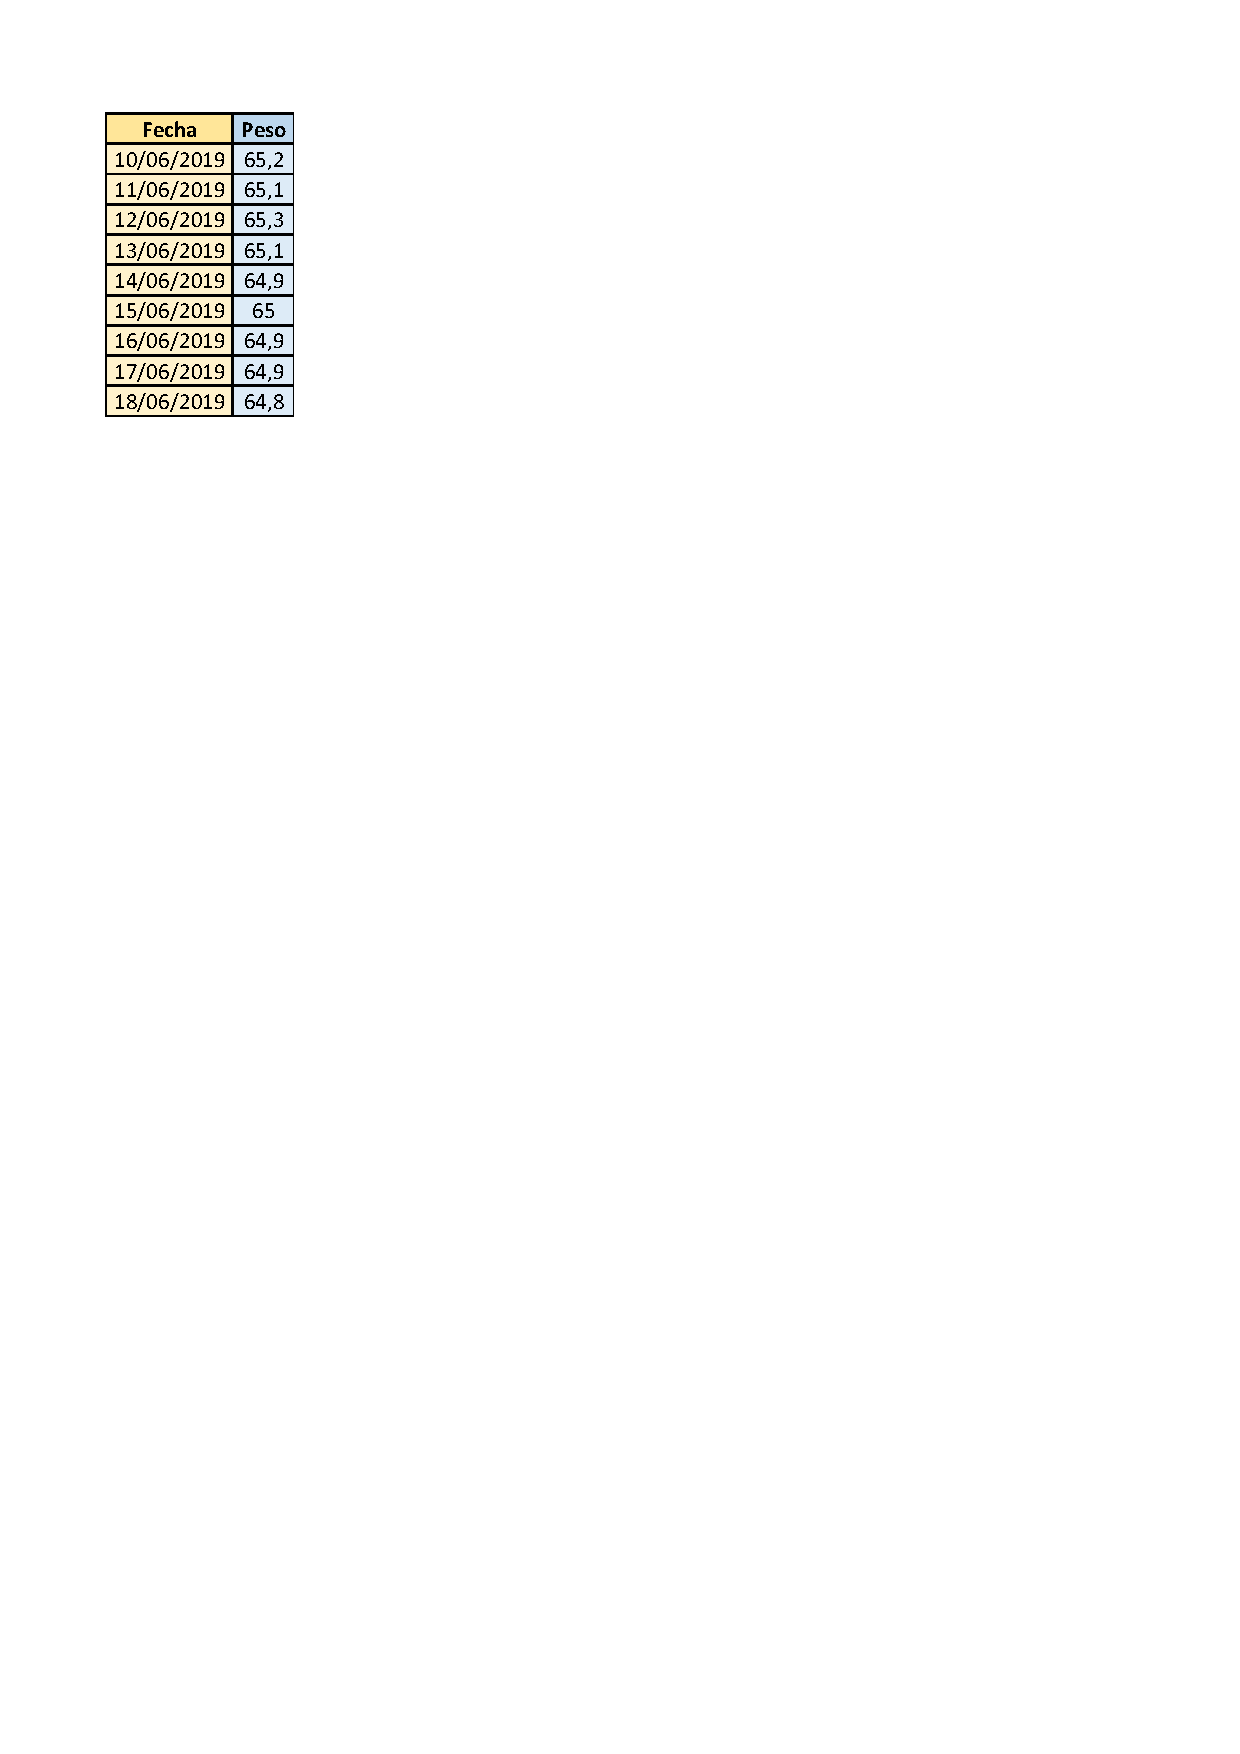
\includegraphics{img/ManejoDeFicherosYDirectorios/MisPesos.pdf}
	\end{figure}
	Los datos que hay en la tabla son exactamente los mismos que hemos introducido.\\
	En el caso de querer leer uno de los ficheros, por ejemplo <<MisNotas.txt>>, lo haríamos de la siguiente forma:
	\\\\\begin{minipage}[c]{0.95\textwidth}
		\lstinputlisting[language=csh,firstline=51,lastline=56]{Programas/FicherosYDirectorios/Program.cs}
	\end{minipage}
	Lo curioso es la asignación, que se hace en el bucle.
	\\\\\begin{minipage}[c]{0.95\textwidth}
		\lstinputlisting[language=csh,firstline=54,lastline=54]{Programas/FicherosYDirectorios/Program.cs}
	\end{minipage}
	Primero asignamos a nuestra variable <<lineaActual>> lo que haya en la línea del fichero que corresponda. Una vez asignado, se evalúa si la cadena resultante no es nula; en el caso de serlo, nos saldríamos del bucle, y en el caso de que no, entraríamos para escribir por consola dicha línea.
	\\\\\begin{minipage}[c]{0.95\textwidth}
		\lstinputlisting[language=csh,firstline=55,lastline=55]{Programas/FicherosYDirectorios/Program.cs}
	\end{minipage}
\chapter{Programación orientada a objetos}
Una correcta programación no es la que realiza la función requerida, sino la que lo hace lo más legible posible; para alcanzar este \textit{Shambhala} de la programación tenemos que echar mano de nuestros amigos: los objetos. Es nuestra labor como programadores saber dividir un programa en partes lógicas, y cada una de esas partes será un objeto.\\
Muchas veces escucharemos la definición de <<objeto>> como una estructura con funciones y métodos, y en gran medida es eso, pero no es algo tan trivial. Un objeto consta, principalmente, de los siguientes elementos:
\begin{itemize}
	\item Campos: serán los tipos de datos que contenga la clase.
	\item Funciones/Procedimientos: son métodos que van dentro de la clase.
\end{itemize}
Pero todo esto se ve mucho mejor con ejemplos; queremos hacer un objeto que sea <<Rally>>. En el objeto irá el nombre del rally, la ubicación, el piloto campeón y la escudería campeona.
\begin{figure}[H]
	\centering
	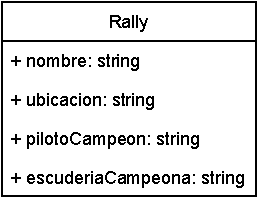
\includegraphics{img/POO/objeto1.pdf}
\end{figure}
Haremos tres objetos <<rally>> y su contenido será el siguiente:
\begin{figure}[H]
	\centering
	\hspace*{-1.5in}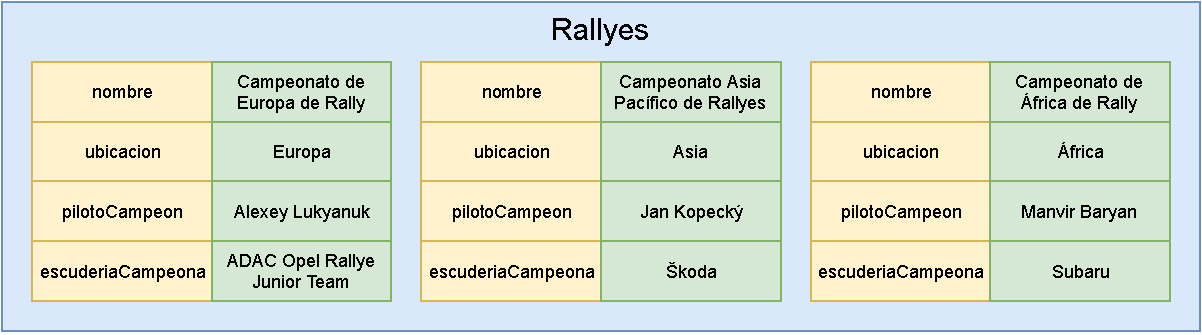
\includegraphics{img/POO/conjuntoObjeto.pdf}
\end{figure}
Ahora que ya sabemos que tenemos que crear los tres objetos <<Rally>>, vamos a ver cómo se hace en código. Primeramente haremos una clase y en ella añadiremos los campos.
\\\\\begin{minipage}[c]{0.95\textwidth}
	\lstinputlisting[language=csh,firstline=5,lastline=8]{Programas/POO/Rally.cs}
\end{minipage}
Ya tendríamos los campos de la clase creados, ahora vayamos al constructor:
\\\\\begin{minipage}[c]{0.95\textwidth}
	\lstinputlisting[language=csh,firstline=10,lastline=17]{Programas/POO/Rally.cs}
\end{minipage}
Y la clase se vería tal que así:
\\\\\begin{minipage}[c]{0.95\textwidth}
	\lstinputlisting[language=csh]{Programas/POO/Rally.cs}
\end{minipage}
En el programa principal haremos una colección de rallyes; en nuestro caso, haremos una lista; podemos introducir los rallyes en la lista de diferentes maneras.\\
Añadiéndolo directamente en la creación de la lista:
\\\\\begin{minipage}[c]{0.95\textwidth}
	\lstinputlisting[language=csh,firstline=13,lastline=19]{Programas/POO/Program.cs}
\end{minipage}
Creando el objeto asignándolo a una variable y metiéndola en la lista:
\\\\\begin{minipage}[c]{0.95\textwidth}
	\lstinputlisting[language=csh,firstline=21,lastline=25]{Programas/POO/Program.cs}
\end{minipage}
Añadiéndolo a la lista instanciando el objeto sin pasar por una variable:
\\\\\begin{minipage}[c]{0.95\textwidth}
	\lstinputlisting[language=csh,firstline=27,lastline=30]{Programas/POO/Program.cs}
\end{minipage}
Y de este modo tendríamos en nuestra lista los tres rallyes metidos.
%Un posible ejercicio sería que cada objeto <<rally>> tuviera un histórico de las victorias y que con indizadores pudieramos acceder a ellas: [nombreRally, año]
\chapter{Indizadores}
Un indizador\cite{msdn:indizador} nos va a permitir tratar como una matriz una clase o una estructura. Para acceder a un elemento de una matriz lo hacemos con el operador <<[ ]>>; si quisiésemos obtener el elemento que hay en el índice 3, lo haremos con <<array[3]>>. Vamos a hacer una modificación en la clase <<Rally>>: en vez de guardar el actual piloto campeón y su escudería, guardaremos un diccionario con una estructura de datos que se llamará <<Equipo>> como valor y un entero (\textit{int}) como clave. La clave será el año en que el equipo ganó. La idea es acceder al equipo ganador con un indizador directamente sobre la clase. La estructura del equipo se vería tal que así:
\\\\\begin{minipage}[c]{0.95\textwidth}
	\lstinputlisting[language=csh,firstline=7,lastline=17]{Programas/Indizadores/Rally.cs}
\end{minipage}
Ahora definamos el comportamiento del operador <<[ ]>> en nuestra clase. Lo haremos de la siguiente manera:
\\\\\begin{minipage}[c]{0.95\textwidth}
	\lstinputlisting[language=csh,firstline=30,lastline=33]{Programas/Indizadores/Rally.cs}
\end{minipage}
Con esto obtendríamos el equipo ganador del año que se introdujera entre corchetes.\\
Y la clase pasaría a ser esta:
\\\\\begin{minipage}[c]{0.95\textwidth}
	\lstinputlisting[language=csh]{Programas/Indizadores/Rally.cs}
\end{minipage}
En el programa principal podremos acceder a la escudería y el piloto que ganó en un rally un año específico de una manera simple, sencilla y <<bonita>>. Para añadir cada uno de los palmareses de las competiciones haremos tres diccionarios, uno para cada competición:
\\\\\begin{minipage}[c]{0.95\textwidth}
	\lstinputlisting[language=csh,firstline=13,lastline=40]{Programas/Indizadores/Program.cs}
\end{minipage}
Y los meteremos todos en nuestra lista de rallyes:
\\\\\begin{minipage}[c]{0.95\textwidth}
	\lstinputlisting[language=csh,firstline=42,lastline=53]{Programas/Indizadores/Program.cs}
\end{minipage}
Y ya podríamos acceder a los ganadores de los rallyes mediante un indizador. Lo usaríamos de la siguiente manera:
\\\\\begin{minipage}[c]{0.95\textwidth}
	\lstinputlisting[language=csh,firstline=55,lastline=57]{Programas/Indizadores/Program.cs}
\end{minipage}
Obtenemos la siguiente salida:
\begin{verbatim}
	Ganador del rally en el año 2015:
	    Piloto: Jaspreet Singh Chatthe
	    Escudería: Mitsubishi
\end{verbatim}
\chapter{Eventos}
Un evento\cite{msdn:evento} no es más que el envío de un mensaje cuando se produce una acción. Dicha acción puede ser causada por el usuario o por otro motivo ajeno a él. Quién provoca el evento es denominado <<emisor del evento>> y lo capturará un manejador de eventos, el cuál le habremos indicado que sea quién maneje el evento que acaba de ser lanzado.
\begin{figure}[H]
	\centering
	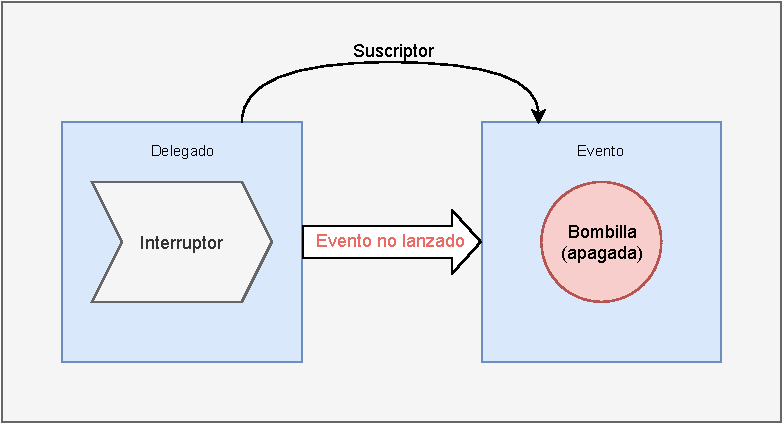
\includegraphics{img/Eventos/eventoEsquema1.pdf}
\end{figure}
El evento que tenemos en la figura superior está esperando que alguien lo llame, y el interruptor está esperando que alguien lo accione para que pueda lanzar el mensaje (lanzar el evento). 
\begin{figure}[H]
	\centering
	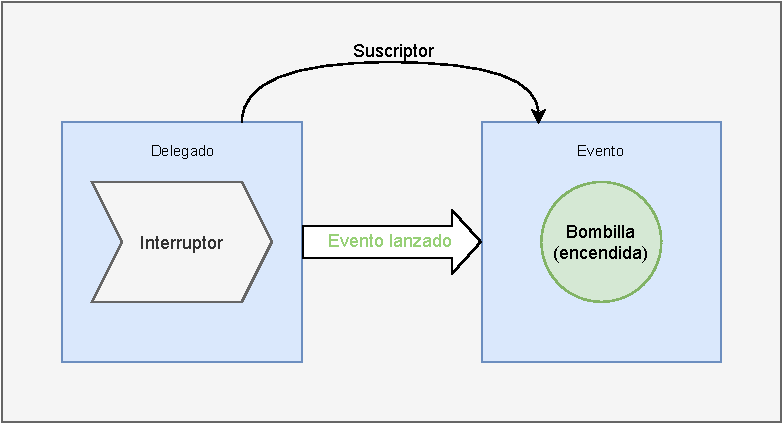
\includegraphics{img/Eventos/eventoEsquema2.pdf}
\end{figure}
Una vez el interruptor se accione el evento se ejecutará porque habrá sido suscrito en el programa. Una suscripción no es más que <<capturar>> esa señal mandada por quién emite el mensaje y una vez capturada ejecutar una función.\\
Hagamos un programa simple: tendremos la bombilla, la cual se nos mostrará su estado en pantalla, y un interruptor, el cual el usuario podrá activar con la pulsación de la letra <<R>> y una vez activo el estado de la bombilla pasará a encendido. Como tenemos el estado de la bombilla en pantalla, veremos cuándo está activada.\\
Crearemos la clase bombilla y en ella definiremos el evento; en el programa principal suscribiremos ese evento a la función que se ejecutará cuando se lance. La clase tendrá un solo campo:
\\\\\begin{minipage}[c]{0.95\textwidth}
	\lstinputlisting[language=csh,firstline=7,lastline=8]{Programas/Eventos/Bombilla.cs}
\end{minipage}
El programa transcurrirá en el siguiente método, dentro de <<Bombilla>>:
\\\\\begin{minipage}[c]{0.95\textwidth}
	\lstinputlisting[language=csh,firstline=12,lastline=27]{Programas/Eventos/Bombilla.cs}
\end{minipage}
De este modo nos será más fácil lanzar el evento; lo lanzaremos en la línea 20.\\
El programa principal es muy simple: 
\begin{enumerate}
	\item Creamos una bombilla
	\item Creamos una función que se adecúe al delegado que habiamos creado
	\item Suscribimos el evento de la bombilla a la función que acabamos de crear
	\item Llamamos al método que hemos creado en bombilla
\end{enumerate}
El programa se verá tal que así:
\\\\\begin{minipage}[c]{0.95\textwidth}
	\lstinputlisting[language=csh]{Programas/Eventos/Program.cs}
\end{minipage}
\begin{itemize}
	\item Línea 7: creación del objeto <<Bombilla>>
	\item Línea 14-17: creación del método
	\item Línea 9: suscripción del método al evento
	\item Línea 11: llamada a la función de <<Bombilla>>
\end{itemize}
\chapter{Tareas}
Una tarea
\chapter*{Definiciones} %\hypertarget{ficheroRet}{\hyperlink{ficheroDef}{fichero}}
\label{ch:definiciones}
\begin{itemize}

	\item \hypertarget{punteroDef}{\hyperlink{punteroRet}{Puntero}}: un puntero puede parecer algo muy complejo de entender. De hecho, en \textit{C}\# no tenemos el tipo de datos <<puntero>> (por suerte o por desgracia). Un puntero no es más que una dirección de memoria. 
	\\AQUÍ UNA FIGURA DE ESAS QUE TÚ Y YO SABEMOS QUE ESTÁN FLAMAS
	
	\item \hypertarget{nodoDef}{\hyperlink{nodoRet}{Nodo}}: dado que viene referido de una estructura de datos, un nodo es un registro dónde se tiene guardado un dato de interés y al menos un puntero que apunte a otro nodo colindante (que sea anterior o posterior). 
	
	\item \hypertarget{directorioDef}{\hyperlink{directorioRet}{Directorio}}: agrupación virtual de ficheros y directorios. Un directorio puede no contener nada, pero un fichero siempre debe estar contenido en un directorio.
	\\FIGURA FLAMANTE DE UN ÁRBOL DE DIRECTORIOS FUA 3.0
	
	\item \hypertarget{ficheroDef}{\hyperlink{ficheroRet}{Fichero/archivo}}: conjunto de \hypertarget{bitRet}{\hyperlink{bitDef}{bits}} que representan información.
	
	\item \hypertarget{bitDef}{\hyperlink{bitRet}{Bit}}: unidad mínima de información. Un bit tiene dos estados: <<0>> y <<1>>. Los bits van contenidos en \hypertarget{byteRet}{\hyperlink{byteDef}{bytes}}.
	
	\item \hypertarget{byteDef}{\hyperlink{byteRet}{Byte}}: Un byte es una agrupación de 8 bits independientes donde el valor de cada bit es esencial para la correcta comprensión de los datos. Del mismo modo que se agrupan los bits para guardar información, se pueden agrupar bytes para poder guardar más aún. Pongamos el ejemplo de un numero entero con signo (\textit{int}) que se representa con cuatro bytes:
	\begin{figure}[H]
		\centering
		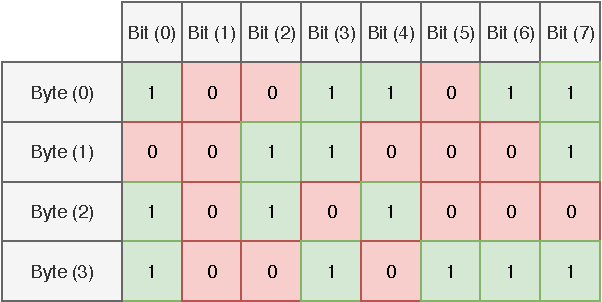
\includegraphics{img/Definiciones/Byte/byte1.pdf}
	\end{figure} 
	El número representado en la figura superior sería el \textit{10011011 00110001 10101000 10010111}$_{2}$ en binario y el \textit{2603722903}$_{10}$ en decimal. Cada uno de los bits tiene una función trascendental en la información que queremos transmitir. Si alteramos un solo bit el número (o dato) que obtengamos será completamente diferente. Por ejemplo, cambiamos el último bit del tercer byte por un <<1>> (\textit{10011011 00110001 1010100\textbf{1} 10010110}$_{2}$); nos daría <<\textit{2603723158}$_{10}$>>, un número completamente diferente.

	\item \hypertarget{codificacionDef}{\hyperlink{codificacionRet}{Codificación}}: \textbf{referido a la codificación de caracteres}, la codificación es la conversión de un carácter (que nosotros consideramos <<lenguaje natural>>, como por ejemplo la letra <<G>>) a un símbolo de otro sistema de representación; como estamos en el campo de la informática, se codifica como un número. Véase \hypertarget{ASCIIRet}{\hyperlink{ASCIIDef}{ASCII}}.
	
	\item \hypertarget{ASCIIDef}{\hyperlink{ASCIIRet}{ASCII}}:
	
	\item \hypertarget{curdirDef}{\hyperlink{curdirRet}{Directorio del proyecto}}:
	
	\item \hypertarget{CSVDef}{\hyperlink{CSVRet}{CSV}}:
		
\end{itemize}

\addcontentsline{toc}{chapter}{Definiciones}

\bibliography{references} 
\bibliographystyle{ieeetr}
\addcontentsline{toc}{chapter}{Bibliografía}
\end{document}